\setlength{\parskip}{.2em}
\graphicspath{ {./chapter-3/figures/} }
\captionsetup[figure]{labelfont=bf}
\captionsetup{margin=1.5em}
\captionsetup[table]{labelfont=bf}


\chapter{Landscape exploration with simple systems}
\label{chapter_3}

%% The following annotation is customary for chapter which have already been
%% published as a paper.
\blfootnote{Parts of this chapter have been published in Applied Optics \textbf{55}, 10449 (2016) \cite{HouSimple16}.}

%% It is only necessary to list the authors if multiple people contributed
%% significantly to the chapter.
%\authors{Albert {\titleshape Einstein}}

% %% The '0pt' option ensures that no extra vertical space follows this epigraph,
% %% since there is another epigraph after it.
% \epigraph[0pt]{
%   A journey of a thousand miles begins with a single step
% }{Laozi}

% \epigraph{
%     Sample quotes
% }{author}

% \begin{abstract}
% Previous researches have shown that different solutions of the optical system can be found using saddle point based method for some simplified cases\cite{PascalTriplet2009}. It is important, however, to study whether the saddle point based method still perform well in practical lens design problems. To study this, we chose to start with a relative simple example.
% \end{abstract}

% %% Start the actual chapter on a new page.
% \newpage

\noindent This chapter is based on \cite{HouSimple16}. We show here that in the design landscape of a wide-angle pinhole lens and in closely related optimization landscapes, all good local minimums found by other methods can be obtained easily with a succession of one-dimensional searches starting from simpler systems. By replacing high-dimensional searches with a succession of one-dimensional searches, the design efficiency can be increased significantly. By combining this method with conventional design methods, the wide-angle pinhole lens can be designed starting from a single lens.

% Reason for choosing the wide-angle pinhole lens. 1) Application wise, it is application wise popular. 2) It is sufficiently different from the previous studied ideal examples.
In a research paper in 2004 \cite{BociortThinLens2004}, Bociort et al. shows that when a thin lens model is used, and the only the spherical aberration is considered, the minima and saddle points in the lens design landscape form a network. The saddle points in this network can be theoretically predicted, hence from the saddle points, minima are obtained. A research conducted in 2009\cite{PascalTriplet2009} claims that there is a fundamental network for a lens design problem with a certain number of lenses. Pascal et al. gives the examples of the fundamental network of doublet and triplet systems. In the paper, the author predicts that in practical design cases, the system shape of the solutions will not exceed the system shapes from the fundamental network. In the later research in 2010\cite{BociortTripletExplained2010}\cite{BociortToyModel2010}, Bociort shows that a toy model based on third-order spherical aberration can be used to mathematically explain the fundamental network of the triplet. 

It seems that given the dominant aberration is spherical aberration, when the thickness of the lenses are not that big, it is possible to predict the existing solutions within the network. However, in practical cases, aberrations other than spherical aberration will also determine the topology of the merit-function landscape. In this case, it is very difficult to build an analytically model to predict the behaviour of the merit-function landscape (if it is possible, it is also easy for the current algorithm to look for alternative solutions).

Despite the difficulty of using analytic model to predict the merit-function landscape, we have shown earlier that in the lens design space a special structure is present that makes the lens design problem different from a general global optimization problem: certain saddle points existing in the landscape are reducible to minimums of simpler systems plus one additional element. Using this structure, we developed a method called saddle-point construction (SPC) \cite{MVTurnhoutSPC15} to obtain new design solutions. Adding a lens element as usual leads after optimization to one minimum. However, by adding a lens with SPC, the resulting saddle-point system will lead to two minimums. When starting from a minimum with $N$ variables, with SPC we can systematically find minimums in an $N+2$-dimensional variable space by using one-dimensional searches, rather than $N+2$-dimensional searches. Important questions are however, how many minimums existing in the landscape can be obtained in this way, by replacing high-dimensional searches with one-dimensional searches? What percentage of them can be found? Can we at least obtain the good solutions? In this chapter, we evaluate the performance of saddle point construction in more general problems, especially in problems of practical interests. 


%%%%%%%%%%%%%%%%%%%%%%%%%%%%%%%%% Section 1 %%%%%%%%%%%%%%%%%%%%%%%%%%%%%%%%%%%%%%%
\section{Wide angle pin-hole lens}

A wide angle pin-hole lens (designed by Irina Livsthis from ITMO) has been chosen to study the design landscape using saddle point construction. This kind of lens becomes very popular in recent years, where they are largely used in surveillance applications. The lens has an aperture stop with a small diameter placed in front of the system. All lenses are in contact, one lens is cemented, and three different glass materials are used [see Figure \ref{fig:widepinLens}(a)]. The specifications are given in Table \ref{table: sysspec}. In Figure \ref{fig:widepinLens}(b) a 2D image simulation made with CODEV shows that, despite its simplicity, the system has an imaging quality that is adequate for its intended purpose. The system can also be adapted for spectral imaging applications \cite{Strauch2015}. For optimization we used the default CODEV merit function that is based on transverse ray aberrations. The value of the merit function (called in CODEV error function) for this system is 5.72.

\begin{figure}[h!]
    \centering
    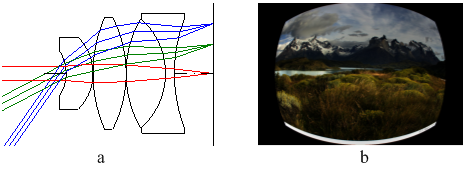
\includegraphics[scale=0.72]{chapter-3/figures/WidePinLens.png}
    \caption{Wide-angle pinhole lens. (a) Lens drawing. (b) 2D image simulation of its imaging quality.}
    \label{fig:widepinLens}
\end{figure}

\setlength{\arrayrulewidth}{.5mm}
\setlength{\tabcolsep}{18pt}
\renewcommand{\arraystretch}{1.2}
\begin{table}[h!]
    \centering
    \captionsetup{justification=centering}
    \caption{System specification}
    \label{table: sysspec}
    \vspace{-1em}
    \begin{tabular}{ p{20em} c }
    \hline 
    Entrance pupil diameter (EPD, mm) & 0.8\\
    Full field of view (FOV, °) & 110\\
    Effective focal length (EFL, mm) & 3.5\\
    Wavelength (nm) & 644, 546, 480\\
    \hline
    \end{tabular}
\end{table}





%%%%%%%% SECONTION Switching %%%%%%%%%%%%%%%%%%%%%%%
\section{Switching between local minima}

To find other possible solutions for the same specifications, two different global optimization methods were used, Global Synthesis from CODEV \cite{KuperGO1992}\cite{RogersGO2006} and a saddle-point detection method (the program NETMIN) developed earlier by us \cite{MarinescuSPD07}. In this example, for simplicity only the surface curvatures were used as variables. Minor edge thickness violations, which can be easily corrected in a later stage, are acceptable in this analysis. 

We are interested to find the stable solutions, i.e., the solutions that do not easily appear or disappear when specifications are changed. Three stable solutions were found, denoted in Figure \ref{fig:wideangleSwitch} by M1, M2, and M3. They exist for a wider range of specifications, e.g., not only for the field of view (FOV) of 110° as shown in Table \ref{table: sysspec}, but also for a FOV of 90°, and not only for an effective focal length (EFL) of 3.5 mm (for which the corresponding merit function values are 5.72, 11.51, and 11.09, respectively) but also for an EFL of 3.0 mm (with merit function values of 6.80, 23.20, and 16.70). These solutions have a reasonable shape, no large edge thickness violation and relatively low merit function values. From the lens drawings of these solutions we observe that the second element differs significantly between them. A few solutions with low stability with large merit function values can also be found, that exist for instance either at EFL 3.5 mm or at EFL 3.0 mm, but not at both. Since these solutions with low stability appear or disappear easily when EFL is changed, it is reasonable to assume that their basins of attraction (i.e., the set of starting points in the variable space that after optimization converge to the given solution) are small and therefore they do not pose a significant danger for trapping the optimization. The solutions with low stability will therefore be ignored in what follows. While no global optimization method can guarantee that all minimums are found, the landscapes examined in this paper are simple enough so that there is a high probability that all minimums having a basin of attraction large enough to be relevant are found with the methods we use. 

\begin{figure}[h!]
    \centering
    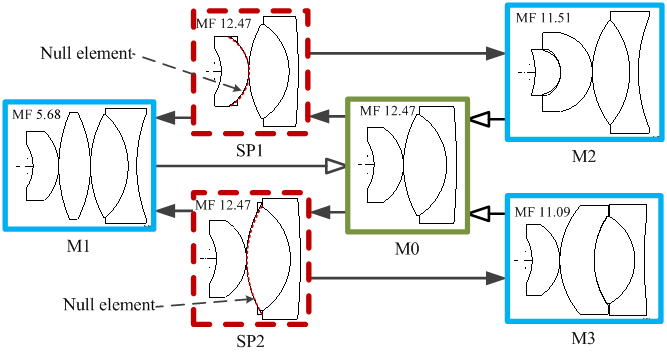
\includegraphics[scale=0.68]{chapter-3/figures/WideAngleSwitch.png}
    \caption{Switching between minimums (blue boxes) using SPC. Extraction of the second element from M1, M2, or M3 results in the system M0 (hollow arrows). Starting from M0, two routes, each having a SP, lead to three different minimums (solid arrows). The two SPs shown in dashed red boxes can be found both by the general and by the special version of SPC. In SP1, the null element has the same curvature as the second surface of M0; in SP2, it has the same curvature as the third surface of M0 (because of two zero thicknesses, we see there three overlapping surfaces, marked by red dashed line).}
    \label{fig:wideangleSwitch}
\end{figure}

Optimization can be trapped in the sub-optimal minimums M2 and M3, which are significantly worse than M1. However, the global minimum M1 can be rapidly obtained with SPC from both of them. In M2 or M3, we extract the second element first and then apply the SPC method (candidates for extraction are in general weaker-power lenses that seem to have no function). After extraction and optimization, both solutions became the M0 system shown in the green box in Figure \ref{fig:wideangleSwitch} Then two SP systems, SP1 and SP2 in Figure \ref{fig:wideangleSwitch}(in the red dashed boxes), were constructed from M0 by adding a null element in between the first and the second lens (i.e., at the position of extraction). From each SP system, two local minimums can be found after optimization. In this case, both SP systems led on one side to the same minimum, the global minimum M1. On the other sides, the two SPs lead to M2 and M3. In fact, from any of these three minimums, the other two can be found by switching. In this example, both ways of using the SPC method described in Section 2 are demonstrated: first, the SPC method can systematically find new solutions with more lenses (M1, M2, and M3) from a simpler system (M0); second, extracting and then adding lenses with SPC can find different minimums in a systematic way. This way of switching between different local minimums is typical for SPC.
%%%%%%%%%%%%%%%%%%%%%%%%%%%%%%%%%%%%%%%%%%%%% Section %%%%%%%%%%%%%%%%%%%%%%%%%%%%%%%%%%%%%%%%%%%%%%%%
\section{Designing a pin-hole system starting from a single lens} \label{chrom90d}

In the previous section we have seen how by using SPC different designs can be found systematically by increasing the number of lenses. By using this approach in combination with traditional methods it is possible to design an optical system starting with just one lens. Here we show how a pinhole lens similar to the one in Figure \ref{fig:widepinLens}(a) can be obtained from a single lens. The specifications are listed in Table \ref{table: sysspec}. We use the same merit function as before.

A global optimization was performed starting from a plane parallel plate. Only one singlet solution was obtained, with MF 576.30, as shown on the left in Figure \ref{fig:WideAngleDesign}(a). This singlet served as a basic element, providing optical power to the system \cite{LivshitsQA2013}. On this singlet SPC was performed by adding a zero-thickness glass element at the back surface. Two doublet minimums were found, with MF 164.81 and MF 1783.94 (the latter one disappears if we replace EFL 3.5 mm by, e.g., EFL 3.0 mm). We chose the better one (the first one) for the next design step. 

\begin{figure}[h!]
    \centering
    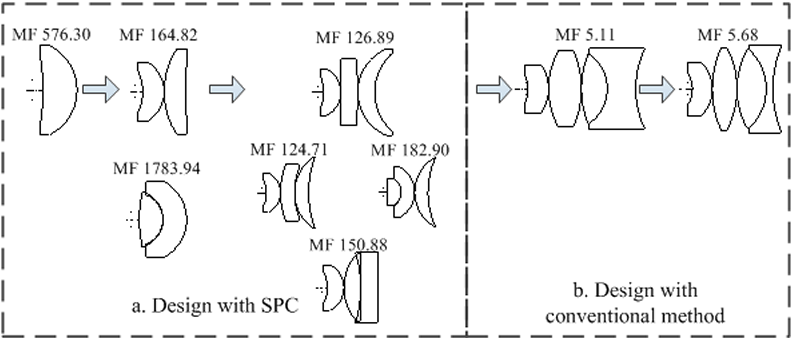
\includegraphics[width=1.0\textwidth]{chapter-3/figures/WideAngleDesign.png}
    \caption{Designing a wide-angle pinhole lens from one lens by combining SPC with conventional methods.}
    \label{fig:WideAngleDesign}
\end{figure}

With the same strategy, SPC was performed on the four different surfaces of the doublet with MF 164.82 and four triplet minimums were found (with merit function values 124.71, 126.89, 150.88, and 182.90, respectively). In the next step, we continue with the best two minimums using conventional design techniques: we change glasses and replace the third lens by a cemented doublet to correct chromatic aberrations. It turned out that the best minimum (MF 124.71) was not useful, because the procedure mentioned above led to ray failure. However, the system with MF 126.89 still remained stable after changing the glass. Optimization with all curvatures and thicknesses as variables led to a system with MF 5.31 [Figure \ref{fig:WideAngleDesign}(b)]. By readjusting the thickness of the lenses for a more compact size, a system with the merit function value of 6.33 was obtained [see Figure \ref{fig:WideAngleDesign}(b)], which closely resembles the system in Figure \ref{fig:widepinLens}(a).

SPC is useful for dealing with minimums created by monochromatic aberrations. It cannot deal directly with minimums created by chromatic aberrations. However, since typically chromatic aberrations are less non-linear than monochromatic ones (e.g., unlike the Seidel aberrations, for axial color the thin-lens expressions are linear), the chromatic aberrations tend to create fewer new minimums than the monochromatic
ones. As shown in this example, in the design process SPC can be easily combined with traditional approaches to handle chromatic correction.


%%%%%%%%%%%%%%%%%%%%%%%%%%%%%%%%%%%%%%%%%%%%% Section %%%%%%%%%%%%%%%%%%%%%%%%%%%%%%%%%%%%%%%%%%%%%%%%
\section{Decomposing a high-dimensional search for new minima in a succesion of one-dimensional searches}  \label{chrom60d}

In the previous section four triplet minimums were found with the SPC method in the search using only one glass, as shown in Figure \ref{fig:WideAngleDesign}(a). Both Global Synthesis and saddle-point detection
(NETMIN) have found only three minimums (missing the one with the merit function value of 182.90). Therefore, in this example the SPC method has the advantage of being able to find more minimums than the two methods used for comparison. However, since in the previous examples the number of minimums found in the landscape is small, in this section we investigate whether the performance of SPC is still good when more minimums are present in the landscape.

In order to generate more minimums, the FOV of the triplet system was reduced to 60° while the other specifications remained the ones given in Table \ref{table: sysspec}. The reason why a reduced
field leads to more minimums will be discussed in the next section.
As in Figure \ref{fig:WideAngleDesign}(a) we only used one type of glass, the variables are only curvatures, we used the same default CODEV merit function, and, for the purpose of this study, we have disabled the control of edge thickness. All lenses are in contact (i.e., all air spaces between lenses are zero). The thicknesses of all lenses in a minimum system are set equal, in order to avoid the multiple appearance of essentially the same minimums (with similar curvatures, but different lens thicknesses) that would unnecessarily complicate the study \cite{HouProc2015}.

For a better understanding of the results, in addition to the comparison of minimums, it is also useful to compare the SPs obtained using SPC with those obtained without a priori knowledge using the (time-consuming) program NETMIN. For SPC we have the option of inserting in the existing minimum either a glass null element (i.e., inserting a lens) or an air null element (i.e., splitting a lens). If we use a zero-thickness glass element, the SPs resulting from the SPC scan will still have a zero-thickness lens, whereas the SPs detected with NETMIN will have finite thicknesses for all lenses. With SPC, the thickness of the zero-thickness glass element is increased once the minimums are obtained from the SPs. However, because in our study all lenses are in contact, the SPs detected with NETMIN will also have zero air spaces. Therefore we decided to study the performance of SPC when air null elements are used. In this case, splitting lenses with SPC leads to SPs with a zero distance between lenses, which are directly comparable with the SPs of NETMIN. For performing SPC with a zero-thickness air element, we first double the thickness of the lens that will be split, re-optimize the system to a minimum, and then insert a zero-thickness air element in the middle of the lens. As we have mentioned in \colorbox{orange}{Section THEORY}, normally both zero-thickness glass and zero-thickness airspace construction may be necessary to obtain more minimums. However, in this example, it turned out that SPC with zero-thickness glass does not reach more results than using zero-thickness airspace. For simplicity and better comparison, we only show the SPC result using zero-thickness airspace.
\begin{figure}[h!]
    \centering
    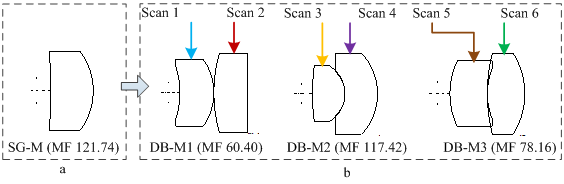
\includegraphics[width=1.0\textwidth]{chapter-3/figures/Single2Double.png}
    \caption{SPC by inserting a zero-thickness air element. (a) Singlet solution. (b) The three doublet minimums that result from the singlet are the starting minimums for the scans shown in Figure \ref{fig:tripletnetwork}.}
    \label{fig:single2double}
\end{figure}
As previously, we started with a single optimized lens [SG-M shown in Figure \ref{fig:single2double}(a)] and obtained with SPC three doublets [shown in Figure \ref{fig:single2double}(b)]. The three doublets DB-M1, DB-M2, and DB-M3 have a total of six lenses. We used each of the six lenses to generate an SPC scan that led to triplet minimums. The colored arrows in Figure \ref{fig:single2double}(b) indicate the lenses that are split (after the thickness doubling that is not shown here) in the corresponding scan.

Figure \ref{fig:tripletnetwork} shows the minimums and SP systems found in the triplet design space with NETMIN and Global Synthesis (Global Synthesis has found nine out of 10 minimums, missing the minimum M6). Five curvatures were used as variables, and the curvature on the last surface was controlled by a \textit{Solve} in CODEV to keep the effective focal length constant.

A significant result of this search is that all 10 triplet minimums shown in Figure \ref{fig:tripletnetwork} were also obtained with SPC starting from the three doublets in Figure \ref{fig:single2double}. Eleven SP systems were obtained from the six one-dimensional SPC scans. Different scans found different numbers of SPs. For instance, in Scan 2 there were four SPs (SP1, SP2, SP7, and SP8 in Figure \ref{fig:tripletnetwork}), whereas in other scans, only one or two SPs were found. The 10 minimums resulted from the 11 SP systems by optimization on both sides of the saddle. Saddle-point systems and minimums obtained from the same scan are connected in Figure \ref{fig:tripletnetwork} with lines having the same color. In the figure, M1 corresponds to the system leading to the final design in the 110° case [MF 126.89 in Figure \ref{fig:WideAngleDesign}(a)]. However, in this case its MF value of 61.14 is not the smallest one in Figure \ref{fig:tripletnetwork}.

NETMIN has found the extra SP system SP12, which cannot be found by SPC. This SP system connects with a dashed link the minimums M3 and M9 in Fig. 8. However, there is sufficient redundancy in the SPC approach, and both M3 and M9 also result from other SP systems which are found by SPC. Therefore the lack of ability of SPC to find SP12 is not critical.

Since we have five variables, with general global optimization tools this search has to be performed in a five-dimensional space. In this example, however, all minimums found with other methods were also found with SPC, where the five-dimensional search was replaced by six one-dimensional searches. Decomposing a high-dimensional search for new minimums in a succession of one-dimensional searches reduces the complexity of the search significantly.

The example discussed above shows the utility of the feature of the optical merit function landscape that enables the decomposition of the search for many of the minimums in simpler steps. This example has the advantage that in this case the feature mentioned above can be observed in a pure form, without interference from other features of the landscape. However, in general other features, which deserve further study for a better understanding, may also play a role. Therefore, it cannot be expected that we can always find all minimums using SPC. However, even when other features are present, SPC can lead to very good results.

For instance, when the search described in Figure \ref{fig:tripletnetwork} was repeated with modified wavelength specifications, SPC found 11 minimums and Global Synthesis found 10 (see Figure \ref{fig:TripletMonoNetwork}). From these minimums, eight, including the best five were found by both methods. For the four minimums that were missed by SPC, two of them are unphysical (minimums 12 and 14, they have either negative or zero back focal length that cannot be corrected, but should be prevented with an additional constraint). These unphysical solutions also have a merit function more than 4 times and more than 50 times of the best solution. The other two minimums missed by SPC (minimums 13 and 15) have a merit function 40 times and 8 times of the best solution. NETMIN found all four solutions missed by SPC, and Global Synthesis found two of them.

\blindtext
\begin{figure}[h!]
  \begin{adjustbox}{addcode={%
    \begin{minipage}{\width}}{%
    \captionsetup{margin=0em}
    \caption{Network of minimums (solid boxes) and SP systems (dashed boxes) in the 60° landscape, where the other specifications are the same as in Table \ref{table: sysspec}. Eleven SP systems result from six SPC scans (each color represents one scan). Optimization starting at these SP systems leads to all 10 minimums that were obtained with NETMIN and Global Synthesis. If in any of these 11 SPs we remove the null element of the corresponding scan (this does not affect the ray paths or the MF), we obtain the starting doublet of the scan. The null elements are marked by crosses with the corresponding color. This figure shows why the lens design landscape is different from general global optimization landscapes: because of the close relationship that exists between local minimums of a design problem (here the 10 triplet minimums) and local minimums with one lens less (here the starting doublets).}\label{fig:tripletnetwork}
    \end{minipage}},rotate=90,center}
    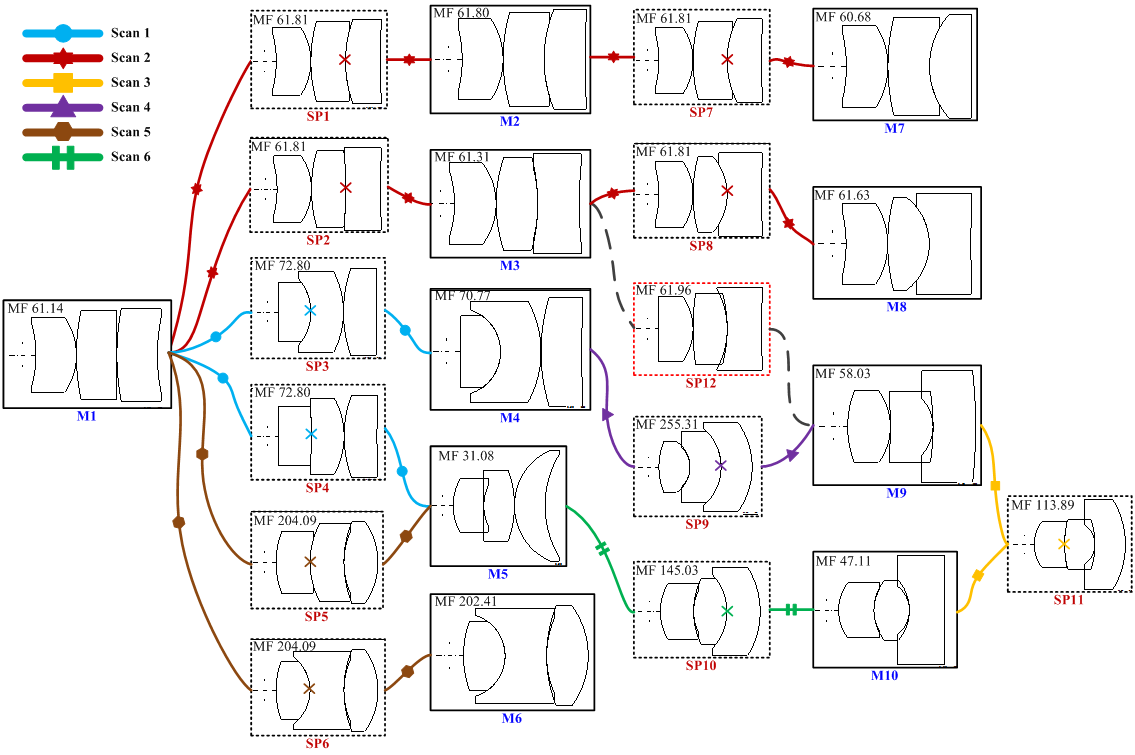
\includegraphics[scale=0.5]{chapter-3/figures/TripletNetwork.png}
  \end{adjustbox}
\end{figure}

Despite the fact that SPC cannot find four (poor-quality) minimums directly, it turns out that by using the switching strategy described earlier we can easily escape from any of them if optimization is trapped there. Eliminating a lens from any of these poor-quality minimums leads to one of the three doublets. From these doublets, better minimums can be obtained with SPC.
\begin{figure}[h!]
    \centering
    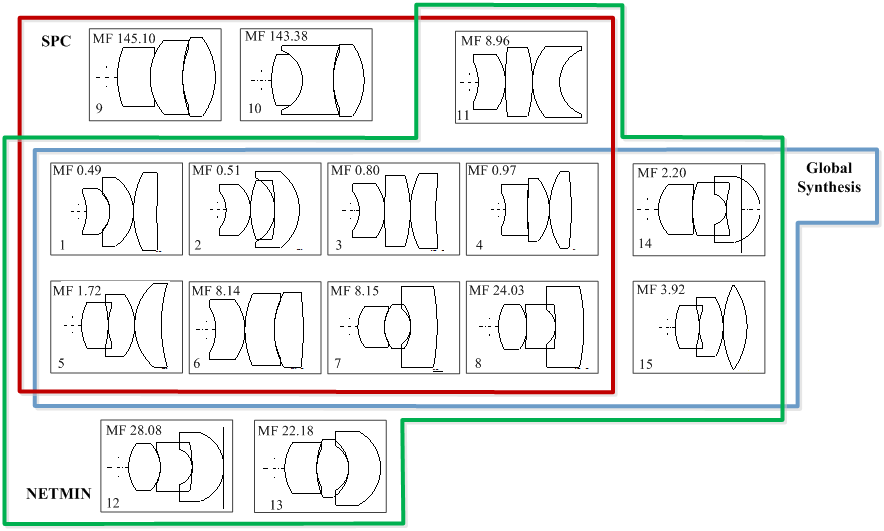
\includegraphics[width=1.0\textwidth]{chapter-3/figures/TripletMoNoNetwork.png}
    \caption{Minimums found with SPC (red box), Global Synthesis (blue box), andNETMIN (green box) in amonochromatic run.Minimums 12 with MF 28.08 andminimums 14 withMF 2.20, whose image planes are inside or coincide with the last lens, are unphysical. The five minimums with the lowest MF value (numbered from 1 to 5) are found by all three methods. Edge thickness violations have been ignored in this search.}
    \label{fig:TripletMonoNetwork}
\end{figure}

However, for understanding the potential and the limitations of SPC it is useful to examine why SPC was not able to reach these four minimums. SPC is based on the assumption that small changes in lens thicknesses do not affect good designs significantly, i.e., that good minimums continue to exist as minimums when a reasonably small non-zero thickness is replaced with zero. This assumption is similar to the one at the basis of the well-known thin-lens aberration theory. In earlier days of lens design, primary aberration formulas using zero thickness were used to predict qualitatively the existence of good designs.

It turns out that the minimums that were not found by SPC only exist for certain non-zero thickness values and do not have a zero-thickness correspondent. However, the existence of these minimums does not contradict our assumption, because these were not among the best solutions. In our numerical experiment, our final solutions have the same thickness for each lens element (1.5 mm). Since in the SPC procedure we increase the thickness of null thickness elements in a minimum, we cannot reach minimums that only exist when the corresponding lens has non-zero thickness. In the NETMIN and Global Synthesis search the lens thicknesses was kept constant. The typical behavior is illustrated in Figure \ref{fig:thicknesschange}(a) and (b). In the system in Figures \ref{fig:thicknesschange}(a) found by SPC, the thickness of the first lens is 1.5 mm. By starting with a zero-thickness null element as the first lens as in Figure \ref{fig:thicknesschange}(b), increasing the thickness leads to the system in Figure \ref{fig:thicknesschange}(a). Also, by decreasing the thickness of the first lens of the system in Figure \ref{fig:thicknesschange}(a), the system in Figure \ref{fig:thicknesschange}(b) is obtained. In contrast, in the system in Figure \ref{fig:thicknesschange}(c) found by NETMIN but not by SPC, when the thickness of the first lens is decreased ray failure occurs and a system with zero-thickness element cannot be obtained. However, systems like the one in Figure \ref{fig:thicknesschange}(c) have low stability. A small perturbation on the system in Figure \ref{fig:thicknesschange}(c) will lead to the system in Figure \ref{fig:thicknesschange}(a).

\begin{figure}[h!]
    \centering
    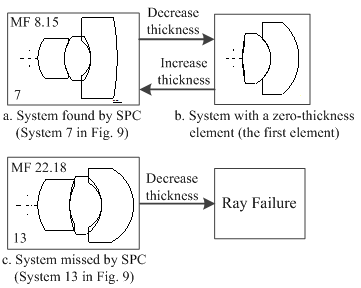
\includegraphics[scale=0.7]{chapter-3/figures/thicknesschange.png}
    \caption{Increasing the thickness of the first element of system (b) results in system (a), and vice versa. System (b), which is obtained by SPC, is a minimum with a zero-thickness element. System (c), which is missed by SPC, does not have a corresponding zero-thickness pair. A small perturbation on system (c) will lead to system (a).}
    \label{fig:thicknesschange}
\end{figure}


%%%%%%%%%%%%%%%%%%%%%%%%%%% Section %%%%%%%%%%%%%%%%%%%%%%%%%%%%%%%%%%%%%%%%%%%
\section{Effect of changing the field of view on the landscape}
In \ref{chrom90d} and \ref{chrom60d} we have seen that when the field of view is reduced, more minimums can be found in the design space. This happens for two reasons. First, when design specifications (e.g., FOV or entrance pupil diameter) are modified, the distances in the design space between minimums and SPs change
and therefore the merit function landscape also changes. As can be observed in numerical experiments, when a minimum and a SP with MI of one collide, they both disappear. Alternatively, such a pair can appear when specifications are changed. Similarly, two minimums with a SP between them can be replaced by one minimum, and two SPs with a minimum between them can be replaced by a SP. This can be explained mathematically by the conservation of topological degree of the MF landscape \cite{vanTurnhoutThesis2009}. A minimum has a topological degree of $1$ and a SP with MI of one has a topological degree of $-1$. The sum of the topological degrees must be conserved when the landscape changes continuously, e.g., by changing the field. Second, when the FOV is increased ray failure appears more easily, and the region of ray failure expands in the design space. Because certain minimums and SPs existing at lower fields cross the border of the ray failure region and disappear, we find fewer of them at large fields.

Using the specification same as the systems in Figure \ref{fig:tripletnetwork}, and varying the FOV, we can see how the number of solutions changes according to the FOV as shown in Figure \ref{fig:FOVvarying}. Three different FOVs are chosen: 110°, 90° and 60°. We obtained six solutions for 110°, five for 90° and ten for 60°. From Figure \ref{fig:FOVvarying}, we can see that some system shapes exist in all the FOV that are chosen. However, other system shapes only exist in specific FOV range.
For FOV 60°, there are five new systems appear, which did not exist for larger field (second row for the 60° systems in Figure \ref{fig:FOVvarying}). The dashed boxes in Figure \ref{fig:FOVvarying} mark the missing correspondent systems which exist in other FOV specifications. As we have mentioned in the previous paragraph, the appearance and disappearance of the systems can be explained by the change of the merit function landscape. This change can be observed from the SPC scan curves.  

\begin{figure}[h!]
    \centering
    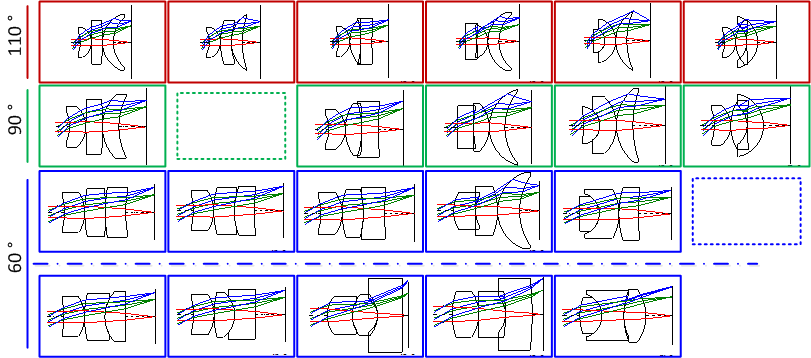
\includegraphics[width=1.0\textwidth]{chapter-3/figures/FOVvarying.png}
    \caption{\colorbox{orange}{For different} field of view, the number of solutions is different. Systems with 110° FOV has six solutions marked by the red colour; Systems with 90° has five solutions marked by the green colour; Systems with 60° marked by the blue colour. The dashed boxes mark the missing systems.}
    \label{fig:FOVvarying}
\end{figure}

\begin{figure}[h!]
    \centering
    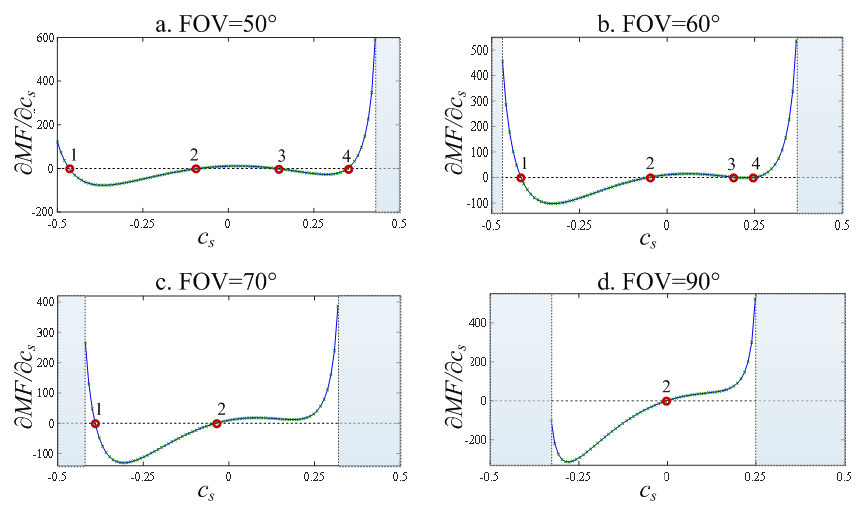
\includegraphics[width=1.0\textwidth]{chapter-3/figures/PhaseTransition_field.png}
    \caption{SPC scan curves for different values of the FOV. Shaded areas are ray failure regions. The scan curves are obtained in the same way as the one shown in \colorbox{orange}{Figure SPSCAN}. Saddle-point curvatures are marked by red circles. With the increase of the FOV, SP 1 disappears in the ray failure region. SPs 3 and 4 merge with the minimum between them, and are replaced by a saddle point (not shown) that is not constructible with SPC.}
    \label{fig:phasechange_field}
\end{figure}

\begin{figure}[h!]
    \centering
    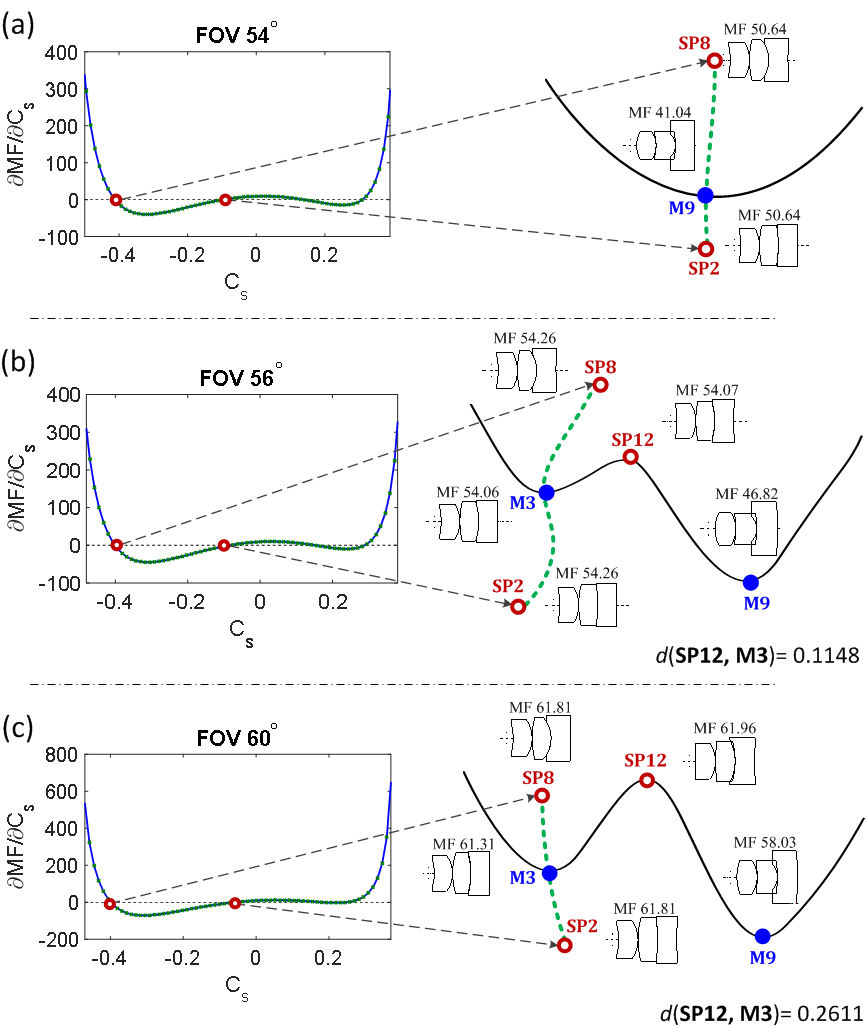
\includegraphics[width=0.8\textwidth]{chapter-3/figures/SystemBorn.png}
    \caption{\colorbox{orange}{how systems appear}}
    \label{fig:systemborn}
\end{figure}

\begin{figure}[h!]
    \centering
    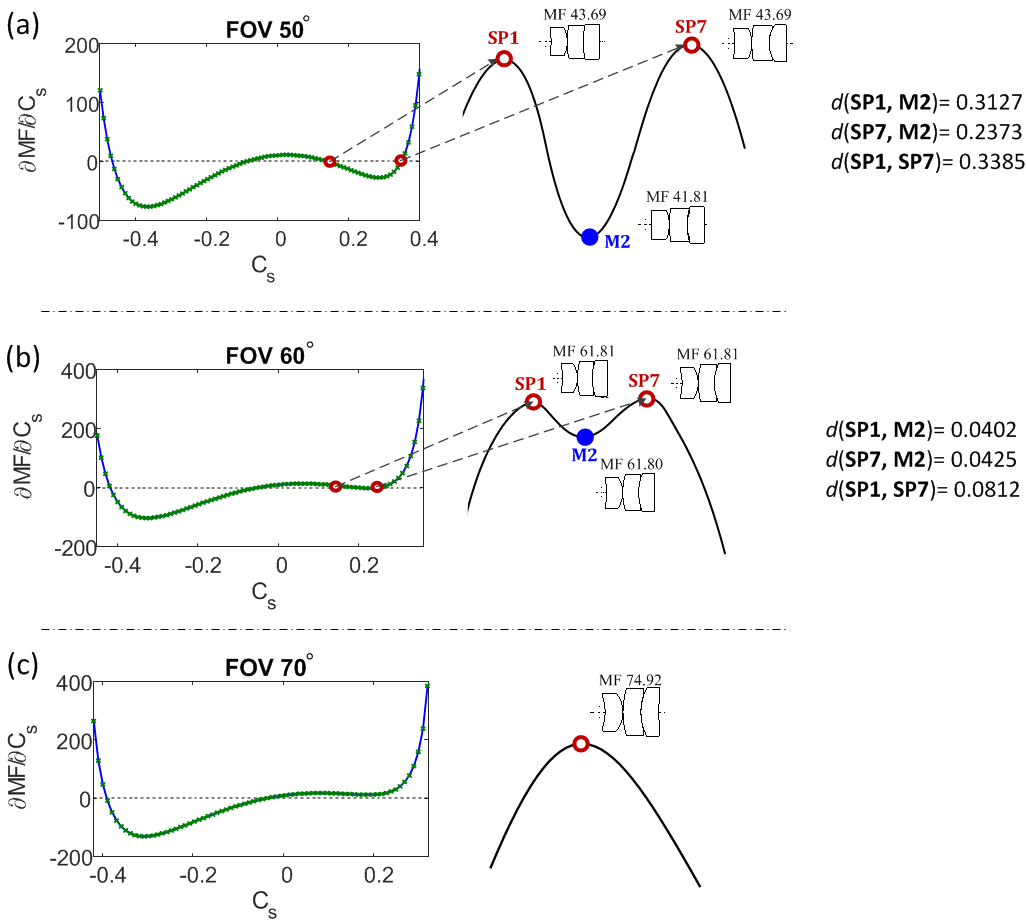
\includegraphics[width=0.8\textwidth]{chapter-3/figures/SystemDie.png}
    \caption{\colorbox{orange}{how systems disappear}}
    \label{fig:systemdie}
\end{figure}

\begin{figure}[h!]
    \centering
    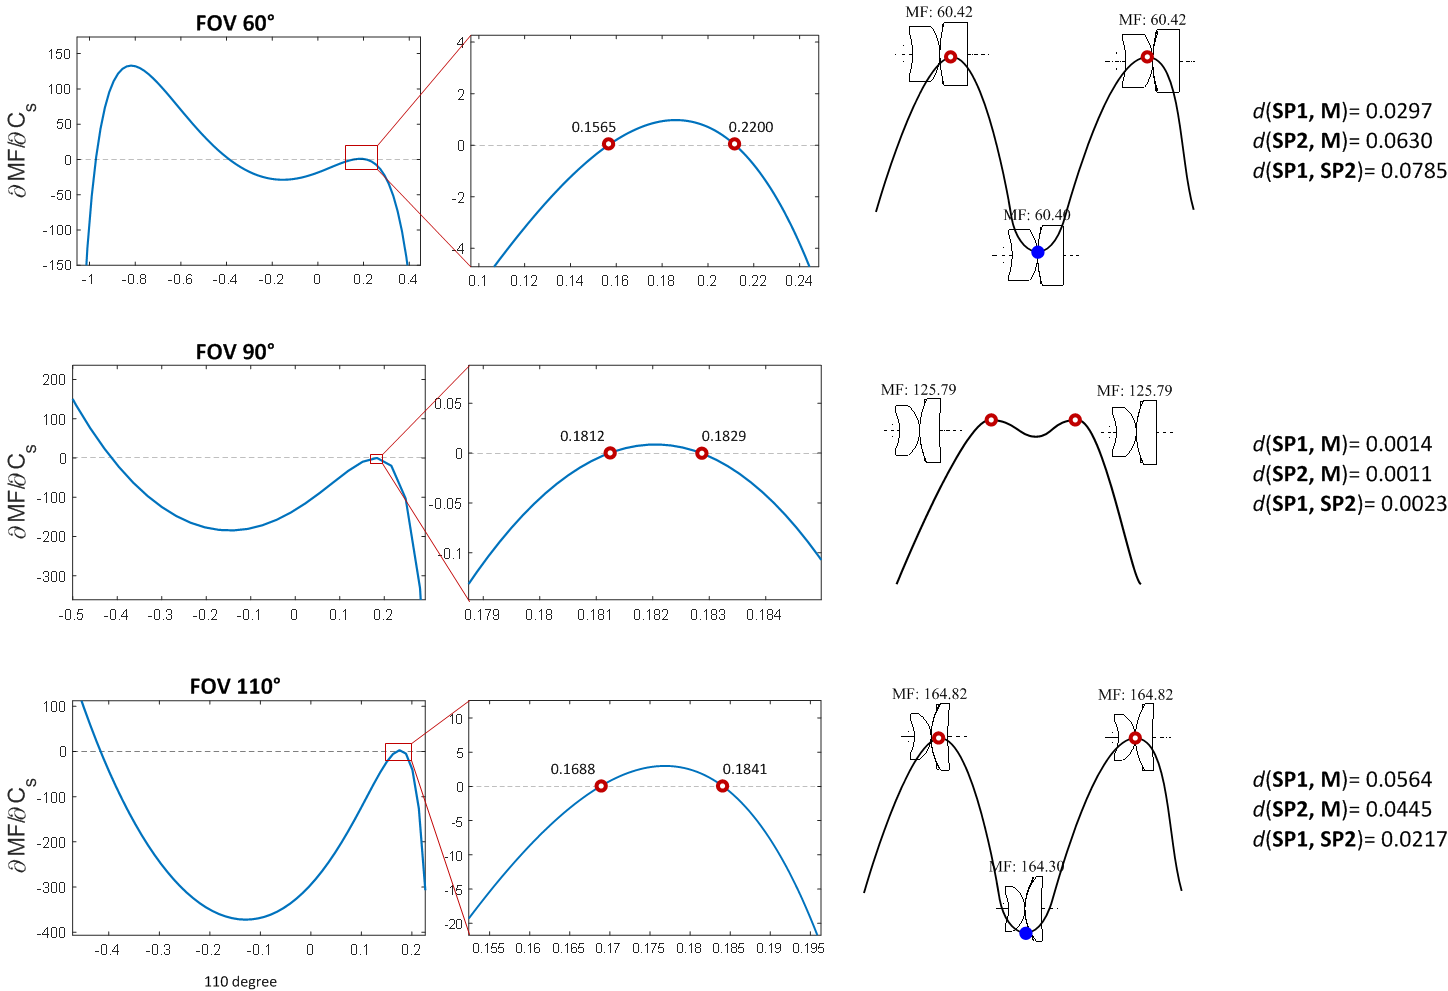
\includegraphics[width=0.8\textwidth]{chapter-3/figures/SystemReborn_vt.png}
    \caption{\colorbox{orange}{how systems reborn}}
    \label{fig:systemreborn}
\end{figure}




These phenomena can also be observed by examining the SPC scan curves. In Fig. 11 the FOV of the system increases from 50° [Figure \ref{fig:phasechange_field}(a)] to 90° [Figure \ref{fig:phasechange_field}(d)]. With the increase of the FOV we observe the expansion of the ray failure region (shown as shaded area). Two SPs are found at 70° [Figure \ref{fig:phasechange_field}(c)], but at 90° [Figure \ref{fig:phasechange_field}(d)] we see that the left SP disappears into the ray failure region.

Also, note another change of the scan curve when the FOV is changed. At 50° [Figure \ref{fig:phasechange_field}(a)] four saddle points can be found. However, at larger fields the third and fourth SP first move closer [Figure \ref{fig:phasechange_field}(b)], merge and then disappear [Figure \ref{fig:phasechange_field}(c) and (d)]. At 50° we found that the last two SPs lead on one side of the saddle to the same minimum. With software written in MATLAB, which communicates with CODEV, we can examine directly, without using SPC, how these critical points change when the field is increased. It turns out that for fields larger than 60°, where the third and fourth SP collide [Figure \ref{fig:phasechange_field}(b)], these two SPs, together with the minimum between them, merge into a single SP. The resulting SP cannot be reduced any more to a simpler local minimum plus a null element and cannot, therefore, be found with SPC. It becomes a usual saddle point, like the saddle points found in general global optimization problems.

%%%%%%%%%%%%%%%%%%% Section %%%%%%%%%%%%%%%%%%%%%%%%%%%%%

\section{original conclusion and discussion}
In this chapter we have studied the design landscape of a wide-angle pinhole lens and its closely related optimization landscapes. However, several observations that result from this study can have a more general validity. Switching between minimums with SPC, as shown in Figure \ref{fig:wideangleSwitch}, can be used in other design tasks as well to avoid the trapping of the optimization in a sub-optimal solution. Combining SPC with conventional design methods, as shown in Figure \ref{fig:WideAngleDesign}, can lead to good complex designs starting from simpler ones \cite{LivshitsSP2014}.

The lens design landscape is different from general global optimization problems because of the close relationship that often exists between the local minimums of a design problem and local minimums with one lens less. Figure \ref{fig:tripletnetwork} is particularly useful to illustrate this structure due to the special choices that were made in the corresponding search (lenses in contact, use of air null elements). The systems SP1–SP11 are triplet saddle points, but if the air null element of the corresponding scan (a pair of surfaces that has no influence at all on the rays or on the merit function) is removed, they become doublet minimums. However, when these doublet minimums with an extra null element are optimized on both sides of the resulting saddle, they lead to the triplet minimums M1–M10. In the search shown in Figure \ref{fig:tripletnetwork}, these 10 triplet minimums are all minimums found in the landscape with other methods that are used for comparison. Earlier we have encountered this structure in a landscape dominated by spherical aberration, but the wide angle examples discussed here show that this structure is much more general.

The example shown in Figure \ref{fig:tripletnetwork} has the advantage that in this case this special structure can be observed in a pure form, without much interference from other features of the landscape. As we have seen in the examples shown in Figure \ref{fig:thicknesschange} and \ref{fig:phasechange_field} other features can also be present, and we cannot always find all minimums using SPC. However, Figure \ref{fig:TripletMonoNetwork} shows an example where even in the presence of additional features of the landscape (see Figure \ref{fig:thicknesschange}) the five solutions with the lowest MF value found with other methods can still be found with SPC.

The example shown in Figure \ref{fig:phasechange_field} is useful for understanding the relationship between landscapes having this special structure that makes reducibility in simpler steps possible and general global optimization landscapes that do not have this structure. The replacement of SPs 3 and 4 in Figure \ref{fig:phasechange_field}(a) by a usual saddle point, which cannot be constructed with SPC, shows that the landscape is locally transformed into a usual global optimization landscape. However, the transition can also happen in the opposite direction: a usual saddle point splits into two saddle points and a minimum in between. Then, if the two new saddle points are constructible with SPC, the decomposition of the search for new minimums in simpler steps could become useful, as shown in this chapter. This observation can perhaps be important for other global optimization problems as well.

For systems that are more complex than those presented in this paper the utility of SPC will be determined by its practical success, rather than by a detailed study of the entire landscape, which becomes difficult. Although in more complex problems we may encounter more design solutions that are not reachable with SPC, the present results suggest that SPC can find good design solutions and can become a useful practical design
tool. The replacement of high-dimensional searches by one-dimensional searches can lead to a reduction of the complexity of the search that can be essential for practical purposes. In computer programs where the search for new solutions is automated, the general version of SPC could be combined with other methods. In the case of the special version of SPC this has already been achieved in the commercial software SYNOPSYS \cite{DilworthSP2012}. Excepting simple problems, no known global optimization method can guarantee finding all (good) solutions in a reasonable time, and SPC is no exception. However, high-quality designs have already been obtained with the special \cite{MarinescuSP2008}\cite{BociortPatent2010} and with the general versions \cite{LivshitsSP2014} of SPC. SPC will be finally validated if many high-quality designs will be obtained in this way.

We have seen that in lens design we can find good solutions with SPC. This method could also be applicable in other design problems where the conditions described in Sections 3 and 4 of \cite{MVTurnhoutSPC15} or in the Appendix of \cite{BociortToyModel2010} are satisfied. In a different multi-parameter optimization problem, if there is a way to construct a
saddle point in the design landscape, then in principle, it should be possible to follow the same procedure as in lens design to search for new solutions.


\references{dissertation}

